We use the NSF ExoGENI cloud testbed~\cite{ExoGENI:web} to create a virtual network for our training data generation. We specifically emulate aspects of the Open Science Grid (OSG)~\cite{OSG:web} data federation network that is highly utilized to distribute data for high throughput scientific computing. Pegasus, a popular WMS to coordinate the data transfer and compute job submission in such an environment, has recently added end-to-end flow level integrity error checking capability~\cite{swip:pearc:2019}.    

In order to simulate different types of sources of integrity errors, we added a new utility in Chaos Jungle~\cite{swip:pearc:2019,chaosjungle:web}, which can corrupt arbitrary file(s) in nodes in addition to packets out of network interfaces according to a given probability. This tool gives us the capability to inject controlled errors into any network elements using several integrity threat models~\cite{threat-model}.

The main design goal here is to automate the experiment creation, configuration, and data collection at any given scale in order to guarantees repeatable experiments at different scales and efficient data manipulation for ML model training.

\subsection{Network creation and configuration}
An arbitrary topology can be created on ExoGENI with nodes in the form of virtual machines (VM) running customized images. In our experimental topology, we use a set of end hosts to emulate the OSG data sources and sinks, a virtual network consisting of core routers emulating the backbone network service providers (Internet2, ESNet, etc.) and access routers emulating the access network service providers (regional research and education networks and campus networks). All nodes are connected with virtual layer-2 links with certain throughput guarantees in the private data plane. The end hosts run an Ubuntu image with our Chaos Jungle fault injection tools. The routers run an Ubuntu image with the Zebra software router and our Chaos Jungle fault injection tools. With our automation software, an experimental system can be easily created with routing configured and network reachability established automatically through the APIs and the template scripting capability provided by ExoGENI.   

\subsection{Data transfer and fault injection}
For every experiment, we attach a controller node that can reach all the nodes in the topology via the management plane interface. The controller is provided a Postboot script that automatically learns the experimental topology, creates a list of end hosts, routers, and links, and populates the end hosts with a set of files for the data transfer.

A user can log into the controller node, modify the experimental configuration files that define the data origin and sink nodes, the list of nodes to introduce storage integrity error, the list of network link interfaces to be disrupted by the Chaos Jungle tool, and the fault injection probability.

Then the experiment software can be started to inject the fault, transfer the data files from the origins, check the integrity at the sinks, and collect the data. This sequence is repeated for every fault specified in the configuration file.

\subsection{Data collection and analysis}
At the last step, all the raw data will be processed and stored in the final result database files with predefined feature columns. Each database entry represents one data transfer with features of the file name, file size, origin, sink, access router, integrity error or not, etc. However, the forwarding path is unknown as it is controlled by the routing control plane process. The final result is exported to a Jupyter notebook environment where all the ML-based data analysis is performed.


%\begin{figure}[!ht]
%\begin{center}
%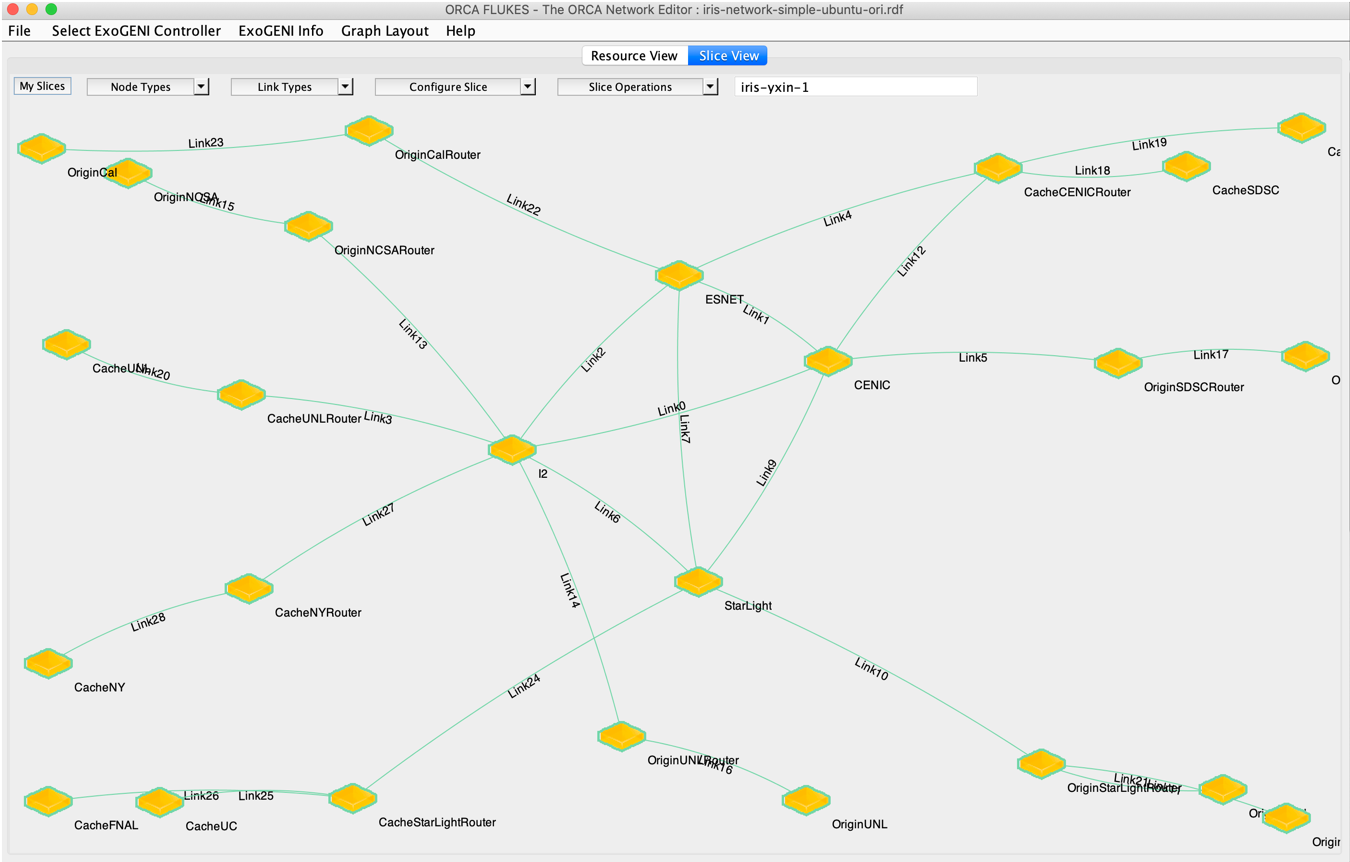
\includegraphics[width=0.48\textwidth]{./figure/experiment-large}
%\end{center}
%\caption{Experimental Topology}
%\label{fig:topology}
%\end{figure}


